%pandoc -f latex -t docx  geospatial-stroke.tex --bibliography references.bib -o geospatial.docx --csl=frontiers-in-physics.csl
\documentclass[utf8]{frontiersHLTH}

\usepackage{url,hyperref,lineno,microtype,subcaption}
\usepackage[onehalfspacing]{setspace}
\usepackage{verbatimbox}
\linenumbers

\def\keyFont{\fontsize{8}{11}\helveticabold }
\def\firstAuthorLast{FirstAuthor {et~al.}} %use et al only if is more than 1 author
\def\Authors{Nicholas Tierney\,$^{1,*}$, Mark Padgham\,$^{2}$, Geoff Boeing\,$^{3}$, David Cooley\,$^{4}$, Michael Sumner\,$^{5}$, Thanh G Phan\,$^{7,8}$ and Richard Beare\,$^{9,10}$}
% Affiliations should be keyed to the author's name with superscript numbers and be listed as follows: Laboratory, Institute, Department, Organization, City, State abbreviation (USA, Canada, Australia), and Country (without detailed address information such as city zip codes or street names).
% If one of the authors has a change of address, list the new address below the correspondence details using a superscript symbol and use the same symbol to indicate the author in the author list.
\def\Address{$^{1}$Laboratory X, Institute X, Department X, Organization X, City X , State XX (only USA, Canada and Australia), Country X \\
$^{3}$School of Public Policy and Urban Affairs, Northeastern University, Boston, Massachusetts, USA\\
$^{7}$Clinical Trials Imaging and Informatics Division of Stroke and Aging Research Group, Monash University, Melbourne, Victoria, Australia\\
$^{8}$Stroke Unit, Monash Medical Centre, Melbourne, Victoria, Australia\\
$^{9}$Department of Medicine, Monash University, Melbourne, Victoria, Australia\\
$^{10}$Developmental Imaging, Murdoch Children's Research Institute, Melbourne, Victoria, Australia}

% The Corresponding Author should be marked with an asterisk
% Provide the exact contact address (this time including street name and city zip code) and email of the corresponding author
\def\corrAuthor{Corresponding Author}

\def\corrEmail{email@uni.edu}

\begin{document}
\onecolumn
\firstpage{1}

\title[Software tools for geospatial analysis]{A review of software tools, data and services for geospatial analysis of stroke services}

\author[\firstAuthorLast ]{\Authors} %This field will be automatically populated
\address{} %This field will be automatically populated
\correspondance{} %This field will be automatically populated

\extraAuth{}% If there are more than 1 corresponding author, comment this line and uncomment the next one.
%\extraAuth{corresponding Author2 \\ Laboratory X2, Institute X2, Department X2, Organization X2, Street X2, City X2 , State XX2 (only USA, Canada and Australia), Zip Code2, X2 Country X2, email2@uni2.edu}

\maketitle

\section{Introduction}\label{introduction}

Treatment of acute stroke involves a complex combination of clinical
services, including emergency dispatch, paramedics, hospital emergency
departments and specialist stroke units. Each of these services
requires careful design in order to deliver best possible care within
the constraints of local geography, government policy and funding
models. In addition, medical research and development is contributing
potential improvements to the possible best care. However changes to
clinical services required to realise potential improvements are
complex and require detailed planning.

Recent advances in acute stroke therapy, in the form of endovascular
clot retrieval
(ECR)\cite{berkhemer2015randomized,goyal2016endovascular,goyal2015randomized,campbell2015endovascular,saver2015stent}
are extremely effective when treatment can be delivered within a
relatively short time window following stroke. This has changed
recently with the publication of the DAWN trial which has pushed the
boundary to 24 hours for clot
retrieval\cite{nogueira2018thrombectomy}. ECR treatment requires
specialist centers with 24 hour staffing by skilled stroke teams and
interventional radiologists with unrestricted access to angiography
suites. Key decisions for governments and policy makers include: how
many centers are required to service a specified area, where should
the centers be placed and what is the expected load on the centers?
Many factors influence the final choice, including the availability of
suitably trained staff, the number of cases required for staff to
retain skills, and costs. It is important, for example, to estimate
whether a single ``hub'' center can service a region, or whether
multiple smaller centers are required to deliver timely
treatment. Furthermore, careful integration of newly operational ECR
hubs with the established thrombolysis (TPA)\cite{tnionda1995tissue}
treatment network is required. Paramedics may potentially deliver
stroke patients to either an ECR or TPA center, and the choice may
have considerable consequences depending on the timing and
pre-hospital large vessel occlusion (LVO) score. In addition,
technical advances, such as mobile stroke units (MSU)[ambulance
equipped with CT scanner and mobile pathology laboratory], improved
prehospital stroke assessments and acute treatment telemedicine
services, increase the number of choices available in, and thus the
complexity of, the acute stroke pathway. For example, suppose funding
is available for $n$ MSUs - where should they be deployed and which
cases should they attend? If a telemedicine services is available,
will the benefits of using it outweigh the risks imposed by the
possible delay in transporting the patient to the ECR hub for definitive therapy? Data are emerging from STRATIS registry that a drip and ship model leads to 99 minutes delay to ECR compared to a direct to mothership approach for cases with large vessel occlusion (LVO) (reference Michael Froehler Circulation 2017).   How will an improved prehospital assessment tool for LVO
change the delivery choices available to paramedics and dispatch
staff? Finally, and possibly most importantly, how do these decisions
reflect the idiosyncracies of a specific city or urban environment?

Time, transport and spatial position are common themes underlying many
of these questions - help must reach a patient, usually via road
transport and in some case air transport, the patient must be assessed and transported to the
``best'' hospital, where the definition of ``best'' relates to both
the transport duration and the services (stroke therapy) available at
the destination hospital. A framework for modelling these scenarios is
valuable in planning and evaluating treatment services and exploring
implications of new technological or treatment choices and changes in
population. In the writing of this review, we have asked several data
scientists to contribute to vignettes to help clinicians and other
data and citizen scientists to become involve in the field. These
contributions take on board the call for paper on geospatial analysis
and transport for this special issue. We have tried to introduce the
topic slowly and include codes in open source software such as R and
Python for reproducibility. These tools are extremely flexible, but
typically involve relatively steep learning curves. We hope that his
article will provide stroke researchers with a useful introduction to
the possibilities offered by these tools. The two examples we present
are a choropleth (thematic map) and a service catchment
basin estimation. A choropleth is a thematic map display in which regions are
coloured by a measure of the region. Choropleths are the workhorse of
geographical visualization. We use demographic and boundary data from
the Australian Bureau of Statistics and incidence data from the
NEMISIS \cite{thrift_stroke_2000,azarpazhooh2008patterns} study to
estimate stroke cases per postcode and display the result on an
interactive map. The service catchment basin estimation involves a
Monte-Carlo simulation of patients attending a rehabilitation service
of 3 hospitals. The catchment basin of each hospital is the region
that has lower travel time to that hospital than any other.  Catchment
basins can be combined with incidence data to estimate load on
rehabilitation centers. The data can be used to explore scenarios,
such as the removal or addition of service centers.

In this article we will introduce these components and provide
examples.

{\em Geospatial analysis} is the the term used to describe modelling
of spatial data. Geospatial analysis has traditionally been the domain
of {\em geographic information systems (GIS)} specialists, employing
commercial software and data products. Recent years, however, have
seen the development of open source tools and free or low cost web
services, such as Google Maps, that make advanced geospatial analysis
accessible and feasible to the non-specialist citizen scientist. In
this article we review a family of computational techniques and
services, collectively termed geospatial analysis tools, that can be
applied to a range of questions relevant to stroke
services. Geospatial analysis tools allow manipulation and modelling
of geospatial data.  These tools, data, and modelling techniques have
a long track record in the quantitative geography, city and regional
planning, and civil engineering research literatures. Geospatial data,
in the context of stroke research, includes the location of patients
and treatment centers, routes through the road network linking
patients to treatment centers, geographic and administrative region
boundaries (e.g.~post codes, government areas, national boundaries)
and disease incidence and demographic information associated with such
regions.

%Geospatial approaches have been used to
%analyse the delivery of emergency clot retrieval services
%\cite{Phan_2017} and to evaluate ``Drip and Ship'' approaches in
%specific locales \cite{Milne_2017} and population level
%access to services \cite{Adeoye_2014}.

%Geospatial tools can be used to analyse and visualise geospatial data,
%such as patient collection location as well as perform a range of
%simulations at varying levels of detail. For example, in
%\cite{Phan_2017}, travel times between a set of randomly generated
%addresses and a set of possible destinations were estimated using
%queries to several Google Application Programming Interfaces (API),
%allowing various configuration of the treatment network to be
%tested. Combination of the resulting catchment areas with demographic
%data allowed loadings to be estimated.

%The studies cited above were constructed using a series of standard
%geospatial analysis components. In this article we will introduce
%these components and provide examples of how they can be used to
%answer health related questions. Examples are implemented using open
%source software, specifically R and python, and source code provided
%so that readers can reproduce and modify them
%\cite{R_Core_Team_2018,sanner1999python,boeing_osmnx_2017}. Geospatial analysis tools
%have traditionally been the domain of specialist commercial software
%and vendors, however this is no longer the case, with a range of open
%source options available to researchers.  These tools are extremely
%flexible, but typically involve relatively steep learning curves. We
%hope that his article will provide stroke researchers with a useful
%introduction to the possibilities offered by these tools.



\section{Background}\label{background}

\subsection{Geospatial frameworks}\label{geospatial-frameworks}

In geospatial analysis, location of a data point in space is referred
in terms of latitude and longitude. More complex data, such as
national boundaries or administrative or postcode boundaries consist
of sets of points connected together in defined orders, typically to
produce a closed shape. Other structures, such as road networks, are
also constructed using sets of points and include other types of
information, such as speed limits, travel direction etc. A geospatial
framework provides mechanisms for representing, loading, and saving
geospatial data and performing fundamental mathematical
operations. For example, the simple features (sf) \cite{Pebesma_2018}
package, on which our R examples are based, provides structures to
represent all manner of shapes and associate them with non spatial
quantities, perform transforms between coordinate systems, display
shapes, compute geometric quantities like areas and distances and
perform operations like intersections and unions. The equivalent
python framework is the geopandas package that provides a geospatial
extension to standard dataframes. A key emerging subdomain of 
geospatial analysis is spatial network analysis. Several open-source 
packages now exist for modeling and analyzing spatial networks, 
such as urban street networks, including dodgr for R (citation) 
and OSMnx for Python \cite{boeing_osmnx_2017}.

\subsection{Sources of regional data}\label{sources-of-regional-data}

The examples below use postcode boundary data available from the
Australian Bureau of Statistics. It is common for boundaries used in
reporting of regional statistics to be available in standard file
formats from the reporting bodies or central authorities along with
the reported statistics. The regional demographics measures, often
derived from national census data, also represent an important source
of information for researchers, including age, sex, income, ethnicity
etc.  For example, in the US, key data sources on sociodemographics
and the built environment include the Census Bureau's decennial census
\cite{us_census_bureau_decennial} (a complete enumeration at fine
spatial scales but coarse, decadal temporal scales), American
Community Survey\cite{us_census_bureau_acs} (a survey
with annual temporal scales, but often fairly large standard errors at
small spatial scales due to the sample size), and TIGER/Line
shapefiles\cite{us_census_tiger_line} of tract,
municipal, and urbanized area boundaries. A comprehensive repository 
of US road network models at regional and municipal scales is available
on the Harvard Dataverse \cite{boeing_street_2019}. Additional regional 
data are frequently available from municipal, state, county, or 
metropolitan governmental agencies.

Demographic data for countries in the European Union are provided by
Eurostat \cite{eurostat}. This includes time series data from several
years to decades on economics, demography, infrastructure, health,
traffic, and more of the EU \cite{Lahti2017}. Geographic data for the
EU is available through the Geographic Information System of the
COmmission (GISCO), part of Eurostat. Similar levels of demographic
data are available from France through INSEE \cite{insee}, Germany
through Destatis \cite{destatis} and, Switzerland through
\cite{swiss-bfs}. There are a number of European sources of geospatial
data - \cite{diva-gis,germany-gis,swiss-3d}.

\subsection{Geocoding and reverse
geocoding}\label{geocoding-and-reverse-geocoding}

Location information, such as a patient home address, is often available
as a street address, rather than a coordinate (a latitude/longitude
pair). However operations, such as plotting addresses on a map, require
a coordinate. Geocoding is the process of converting an address to a
coordinate. Reverse geocoding converts a coordinate to an address. A
coordinate is useful in many other types of computation, as we shall see
in the examples below.

There are two common approaches to geocoding and reverse geocoding. The
most ubiquitous is via web services such as Google Maps. Other services,
such as OpenStreetMap's Nominatim web service and OpenCage
(\url{https://opencagedata.com/}), provide similar capabilities and all
can be queried in a automated way from R and python \cite{opencage}. The
other approach is via a local database of geocoded addresses. One
example, for Australia, is the PSMA (formerly Public Sector Mapping
Agencies) address database available in an R queryable form. A local
database allows many high speed queries, but is often less flexible in
terms of query structure than the web services. Web services are
discussed in more detail below.

\subsection{Distance and travel
estimation}\label{distance-and-travel-estimation}

A key part of a number of studies cited above is the estimation of
travel time between patient and treatment center. The popularity of
personal navigation systems in smartphones has driven the development of
extremely sophisticated tools to estimate the fastest route between
points. One of the best known, Google Maps \footnote{the two APIs
involved are the directions api and distance api}, uses a combination
of information about the road network, historic travel time data derived
from smartphone users and live information from smartphones. The travel
time estimates are thus sensitive to time of day, weather conditions and
possibly traffic accidents. Google, and other web services for travel
time estimation, can be queried in a similar fashion to the geocoding
services. It is also possible to create a local database to represent
the road network, allowing more rapid querying, but losing some of the
benefits of traffic models.

\subsection{Visualization}\label{visualization}

Two forms of visualization are used in the following examples - static
and interactive. Static maps are required for printed reports and
typically present a carefully selected view. Interactive maps allow
exploration of a data set, via zooming and toggling of overlays.
Interactive maps often use web services to provide the background map
``tiles'', over which data is superimposed. Different interactive web
services specialise in different types of display. Some tools produce
static and interactive displays in very similar ways.

\hypertarget{introduction-to-web-services}{%
\subsection{Introduction to web
services}\label{introduction-to-web-services}}

Web services providing various forms of geospatial capabilities are a
crucial component of the geospatial analysis tools now available to
researchers. Web services deliver what used to be complex and
specialised information products to the general public. Geocoding and
travel time estimation two common examples that have already been
discussed. Other capabilities include delivery of tiled maps (such as
the Google Map display), street network and building footprint data
(such as from OpenStreetMap), and census data on sociodemographic or
built environment characteristics (such as from the US Census Bureau's
web site).

\subsubsection{Application programming interfaces
(API)}\label{application-programming-interfaces-api}

Web services are accompanied via an API. The API allows software tools,
such as R or python, to make requests to the web service and retrieve
results. Thus, if we consider the Google Map example, not only can a
user access a map query for an address via a web browser, but a program
can submit the same request. Furthermore, a program can submit a series
of automated requests. For example, given a list of addresses, it is
relatively simple to generate an R or python procedure to geocode all of
them via a web service.

The ability to use APIs in automated methods also leaves them open to
abuse. In addition, many APIs are commercial products and thus charge
for use, although the use is often free for small volumes.

The combination of these factors tends to mean that many APIs require
somewhat complex setup, typically via signup and creation of keys. Terms
of use may evolve over time, with charging being introduced, possibly
leading to a need to enter credit card details.

We have endeavoured to create examples that do not require keys,
simplifying getting started. However, some extensions have been included
that do require keys. These are described in supplementary material.

\subsubsection{OpenStreetMap (OSM)}\label{openstreetmap-osm}

OSM (\url{https://www.openstreetmap.org/}) is a service collecting and
distributing crowdsourced geospatial data. Many useful OSM services are
available without API keys, and it is thus the platform of choice for
examples in this paper. OSM is also unusual in that allows access to
geospatial structures, such as road networks, rather than images
generated from those structures. This capability is used to estimate
travel time.

\subsubsection{Access to the examples}\label{access-to-the-examples}

The examples are available in their source code form from (github).
``Live'' versions are available at (githubpages) and can be viewed in
conjunction with the methods section. The description focuses on the R
versions of the examples. Code is visible in the shaded boxes, while
output of the code, such as maps, are displayed immediately after the
code. Python versions are provided and implement equivalent steps.
Details on downloading and running the examples are available in
supplementary material and at the web site.

\section{Methods}\label{methods}

\subsection{Example 1: Choropleth to visualize estimated stroke
numbers}\label{example-1-choropleth-to-visualize-estimated-stroke-numbers}

\subsubsection{Overview:}\label{overview}

We demonstrate accessing and using different data sources. The first is
Australian Bureau of Statistics census data provided at the postcode
level for population information, stratified by age, as well as postcode
boundary information. The second data source is incidence data from the
North East Melbourne Stroke Incidence Study (NEMESIS)\cite{thrift_stroke_2000}. This is combined
with the first dataset to estimate per-postcode stroke incidence. We
demonstrate geocoding by finding the location of a hospital delivering
acute stroke services, and then display postcodes within 15km, colouring
each postcode by estimated stroke incidence.

The steps involved are described in Table \ref{tab:exampleA}.

\subsubsection{Example 2: Service regions for stroke
rehabilitation}\label{example-2-service-regions-for-stroke-rehabilitation}

In the second example we demonstrate the idea of estimating catchment
basins for a set of three service centers. The idea can be easily
extended to more service centers. A catchment basin, or catchment area
for a service center is the region that is closer to that service center
than any other. The definition of ``closer'' is critical in this
calculation, with travel time through the road network being a useful
measure for many practical purposes. The approach used in this example
involves the sampling of random addresses within a region of interest
around the service centers, estimation of travel time from each address
to each service center, assignment of addresses to the closest service
center, combination of addresses based on service center to form
catchment areas. The catchment areas can then be used to estimate
loadings on service centers.

The first four steps, 1) Loading census and boundary data, 2) Geocoding
service center location and 3) Combining demographics and spatial data
are the same as the previous example, with addresses of multiple service
centers being geocoded. The additional steps are:

\section{Results}
Complete versions of the examples are illustrated online at {\em our
  url} and can be downloaded, run and explored by the reader.

\subsection{Example 1: Choropleth to visualize estimated stroke numbers}
Spatial data, as displayed by an {\em R} session, is illustrated in
Tables \ref{tab:GeocodeMMC} and \ref{tab:MMC20}. Table
\ref{tab:GeocodeMMC} shows the result determining the hospital
coordinates via geocoding, while a subset of the combined spatial,
demographic and estimated stroke count data is illustrated in Table
\ref{tab:MMC20}. A visualization of straight-line distance between
each postcode and the hospital, useful for verifying the calculation
is sensible, is illustrated in Figure
\ref{fig:DistanceToMMC}. Finally, Figure \ref{fig:choropleth} provides
a screenshot of the interactive choropleth featuring postcodes in the
vicinity of the hospital coloured by estimated stroke case load. The display
can be exported as a web page and viewed interactively, with the ability to
pan and zoom and switch display layers on and off.

\subsection{Example 2: Service regions for stroke rehabilitation}
Results of geocoding rehab center addresses is shown in Table
\ref{tab:georehab} with the corresponding visualization in Figure
\ref{fig:RehabCenterLocations}. A small selection of random addresses
is available in Table \ref{tab:headpsma} and the complete set is
visualized in Figure \ref{fig:RehabCenterRandomAddresses}. Boundaries
of postcodes of interest are shown in Figure
\ref{fig:RehabCenterPostcodes}. Figures
\ref{fig:RehabCenterAddressCatchments},
\ref{fig:RehabCenterPolyCatchments} and fig:RehabCenterRoadCatchment
show addressed-based, polygon-based and road-based views of the
computed catchment basin. Figures
\ref{fig:RehabCenterAddressDistanceHex} and
\ref{fig:RehabCenterAddressDistance} show alternative visualizations
of travel time using a hexagonal height map and a colour coded road
network.

Finally, allocation of random addresses to rehabilitation centers and
estimated case loads per catchment center are available in Tables
\ref{tab:rehabrandomassignment} and \ref{tab:rehabcaselaod}

\section{Discussion}\label{discussion}

These examples illustrate fundamental geospatial computational
components in R and python. This includes geocoding with databases and
web services, interactive and static visualization. It also includes
geometric computation of areas and distances, and geospatial
computations of travel time.

The examples in this article illustrate the use of a range of components
that underpin geospatial analysis. By providing an accessible
introduction to these areas, clinicians and researchers can create code
to answer clinically relevant questions on a topics such as service
delivery and service demand. Importantly, these factor in key features
of transport and travel time.

Some points - we've used simple straight-line distances to designate
our region of interest. It is feasible to use either road network or
travel time distances instead, based on the tools presented.

\section{Supplementary Material}\label{supplementary-material}

\subsection{API Keys}\label{api-keys}

Online services which offer an interface to their applications will
sometimes require use of an API key, or application programming
interface key. This key should be unique for each user, developer or
application making use of the service as it is a way for the provider to
monitor and, where applicable, charge for use.

Two major mapping platforms that require an API key are Google Maps and
Mapbox. At the time of writing both allow unrestricted use of the
mapping API. However, Google has limits on the other services it offers
such as geocoding and direction services.

Setting up API Keys for examples

\section*{Table captions}

\begin{table}[h]
\begin{center}
  \sffamily
  \tiny
\begin{enumerate}
\def\labelenumi{\arabic{enumi}.}
\item
  {\bf Loading census and boundary data:} Data from the 2016 Australian
  National Census is available from the Australian Bureau of Statistics
  (\url{https://datapacks.censusdata.abs.gov.au/datapacks/}) , and
  copies are included with examples. The two parts of the data are the
  national postcode boundaries (loaded with the sf::read\_sf command)
  and the demographics, by postcode, for the state of Victoria, loaded
  with the readr::read\_csv command.
\item
  {\bf Geocoding hospital location:} The coordinates of the hospital of
  interest, Monash Medical Centre, are determined by geocoding the
  hospital address, using the tmaptools::geocode\_OSM command. This
  command uses the OpenStreetMap Nominatim geocoding service.
\item
  {\bf Combine demographics and spatial data}. An important feature of the
  simple features and geopandas frameworks is the ability to combine
  spatial data, such as postcode boundaries, with associated statistical
  summaries (stroke count, demographics etc). This step uses the
  right\_join function to attach the demographic data to the set of
  postcodes. The right\_join performs two tasks - attaching the
  demographics data and discarding the postcodes for which we don't have
  demographics data (i.e.~those from other states of Australia).
\item
  {\bf Compute per-postcode stroke incidence:} A column representing stroke
  incidence per postcode is added to the demographics table. The
  computation uses incidence data published by the NEMISIS\cite{thrift_stroke_2000}
  study to provide rates per 100000 for various age ranges. The
  demographics data also includes population by age range, allowing
  computation of stroke incidence as a weighted sum of population
  columns. Names such as Age\_55\_64\_yr\_P refer to the name of a
  column in the demographics table.
\item
  {\bf Compute distance from postcode to hospital:} We create a column
  containing the distance from each postcode to the hospital of interest
  using the sf::st\_distance function, which automatically accounts for
  complexities, such as the curvature of the earth. We also set the
  units of quantities to km. We then use the distance in a simple,
  static, choropleth to verify the operation. Cool colours,
  corresponding to small distances are in the expected location.
\item
  {\bf Discard remote postcodes:}. Postcodes further than 20km from the
  hospital are discarded by filtering the data based on the newly
  calculated distance column.
\item
  {\bf Interactive display of the result:} Finally, an interactive map is
  created using the tmap package. The postcode boundaries are coloured
  according to our estimated stroke count and overlaid on a zoomable map
  provided by OpenStreetMap. Any column in our dataset can be visualized
  in a similar way. A number of useful interactive features are
  available in this style of display, including popup displaying the
  postcode when hovering the mouse over a region and more detailed
  information available when clicking on a region.
\end{enumerate}
\end{center}
\caption{Steps in computation of interactive display of choropleth of
  estimated stroke incidence. \label{tab:exampleA}}
\end{table}

\begin{table}[h]
\begin{center}
  \sffamily
  \tiny
\begin{enumerate}
  \def\labelenumi{\arabic{enumi}.}
  \setcounter{enumi}{3}
\item
  {\bf Compute distance to each service center from each postcode:} A study
  area is generated by computing the distance to each service center
  frome each postcode and retaining only postcodes within 10km of a
  service center
\item
 {\bf Randomly sample addresses in postcodes:} A set of random addresses is created for each
  postcode by randomly sampling a database of addresses. The number of
  addresses sampled depends on the sampling approach and the subsequent
  computations, but if local methods are used it is feasible to use
  large numbers of samples. In this case we use 1000 per postcode. Lower
  numbers would be appropriate if subsequent computations required
  charged web services.
\item
  {\bf Display sample addresses and postcodes:} Display the samples in a map
  form to verify that the distribution matches expected population
  distribution - i.e that there are lower densities in rural areas, and
  that the study area is appropriate.
\item
  {\bf Create a street network database:} In this example we are employing a
  local approach to travel time estimation. The first step is to fetch a
  road network database from OpenStreetmap and convert to a network form
  for analysis. There are a number of tricks discussed in the online
  document that reduce the size of the download by exploiting knowledge
  of the study area.
\item
  {\bf Estimation of travel time:} travel time from each address to each
  service center is then computed using the dodgr::dodgr\_dists
  function, which is optimised to rapidly compute large sets of pairwise
  distances.
\item
  {\bf Address-based catchment basins:} Each address is assigned to a service
  center by identifying the center with the shortest travel time. A view
  using a scatter plot of points coloured by destination is then created
  to verify the result.
\item
  {\bf Polygon catchment basins:} We convert the pointwise classification to a
  polygon representation using a Voronoi tessellation approach. The
  Voronoi tessellation of a set of points is a set of polygon catchment
  basins, one basin for each point. However the definition of ``closer''
  for the Voronoi basins is based on Euclidean distance rather than road
  network distance or travel time. The Voronoi polygons are from
  addresses assigned to the same service center are then merged to
  create the polygon representation of the service center catchment,
  which can be displayed.
\item
  {\bf Estimate caseload per center:} The catchment areas can be used in
  conjunction with the per postcode demographics to make estimates. We
  use our per postcode stroke estimate procedure from the previous
  example as a basis for determining the number of rehabilitation cases
  (a simplification for illustration purposes). The sampled addresses
  are the basis for this computation, with the proportion of sampled
  addresses from a postcode assigned to a service center corresponding
  to the proportion of cases from that postcode attending the center.
\end{enumerate}
\end{center}
\caption{Steps in computation of catchment basin and case load for
  rehabilitation centers. \label{tab:exampleA}}
\end{table}

\begin{table}[h]
\small
\begin{verbnobox}[\fontsize{6pt}{6pt}\selectfont]
Simple feature collection with 1 feature and 7 fields
geometry type:  POINT
dimension:      XY
bbox:           xmin: 145.1207 ymin: -37.92093 xmax: 145.1207 ymax: -37.92093
epsg (SRID):    4326
proj4string:    +proj=longlat +datum=WGS84 +no_defs
                                                query       lat      lon   lat_min   lat_max  lon_min  lon_max                   geometry
1 Monash Medical Centre, Clayton, Victoria, Australia -37.92093 145.1207 -37.92098 -37.92088 145.1207 145.1208 POINT (145.1207 -37.92093)
\end{verbnobox}
\normalsize
\caption{Geocoding results for emergency hospital (Monash Medical Center).\label{tab:GeocodeMMC}}
\end{table}

\begin{table}[h]
\begin{verbnobox}[\fontsize{6pt}{6pt}\selectfont]
Simple feature collection with 6 features and 4 fields
geometry type:  MULTIPOLYGON
dimension:      XY
bbox:           xmin: 144.9055 ymin: -37.85553 xmax: 144.9914 ymax: -37.79821
epsg (SRID):    4326
proj4string:    +proj=longlat +datum=WGS84 +no_defs
# A tibble: 6 x 5
  POA_NAME Tot_P_P stroke_count_est… DistanceToMMC                             geometry
  <chr>      <int>             <dbl>          [km]                   <MULTIPOLYGON []>
1 3000       37975            24.7        15.77496 (((144.9576 -37.79972, 144.9588 -37
2 3002        4964            16.8        15.87279 (((144.9732 -37.80792, 144.9826 -37
3 3003        5515             5.14       18.86105 (((144.9165 -37.79821, 144.9257 -37
4 3004        9307            28.1        14.13294 (((144.985 -37.84569, 144.9842 -37
5 3005         525             0.578      18.11235 (((144.9479 -37.82339, 144.948 -37.
6 3006       18808            20.5        16.57805 (((144.956 -37.82305, 144.9579 -37.
\end{verbnobox}
\caption{Subset of simple features (sf) table containing both demographic and postcode boundary information for postcodes within 20km of the emergency service center. Colums displayed are postcode name, total population, estimate number of stroke cases, distance to emergency center and the postcode geometry. The estimate of stroke cases was based on a combination of population age bands (not illustrated) and incidence data from the NEMISIS study. The distance column was computed between the geometry column of this table ant he geometry column of the geocoded hospital locaiton using the {\em sf::st\_distance} function.\label{tab:MMC20}}
\end{table}

\begin{table}[h]
\begin{verbnobox}[\fontsize{6pt}{6pt}\selectfont]
Simple feature collection with 3 features and 7 fields
geometry type:  POINT
dimension:      XY
bbox:           xmin: 145.0797 ymin: -38.04446 xmax: 145.3457 ymax: -37.95604
epsg (SRID):    4283
proj4string:    +proj=longlat +ellps=GRS80 +towgs84=0,0,0,0,0,0,0 +no_defs
                                                                query       lat      lon   lat_min   lat_max
DandenongHospital   Dandenong Hospital, Dandenong VIC 3175, Australia -37.97611 145.2178 -37.97728 -37.97545
CaseyHospital            62-70 Kangan Dr, Berwick VIC 3806, Australia -38.04446 145.3457 -38.04539 -38.04446
KingstonHospital  The Kingston Centre, Heatherton VIC 3202, Australia -37.95604 145.0797 -37.95830 -37.95344
                   lon_min  lon_max                   geometry
DandenongHospital 145.2162 145.2198 POINT (145.2178 -37.97611)
CaseyHospital     145.3456 145.3457 POINT (145.3457 -38.04446)
KingstonHospital  145.0768 145.0810 POINT (145.0797 -37.95604)
\end{verbnobox}
\caption{Geocoded locations for the 3 rehabilitation centers.\label{tab:georehab}}
\end{table}

\begin{table}[h]
\begin{verbnobox}[\fontsize{6pt}{6pt}\selectfont]
Simple feature collection with 6 features and 13 fields
Attribute-geometry relationship: 13 constant, 0 aggregate, 0 identity
geometry type:  POINT
dimension:      XY
bbox:           xmin: 145.0398 ymin: -37.89162 xmax: 145.0865 ymax: -37.86661
epsg (SRID):    4283
proj4string:    +proj=longlat +ellps=GRS80 +towgs84=0,0,0,0,0,0,0 +no_defs
  POSTCODE ADDRESS_DETAIL_INTRNL_ID STREET_LOCALITY_INTRNL_ID BUILDING_NAME LOT_NUMBER FLAT_NUMBER
1     3145                 11867025                    590471          <NA>       <NA>         126
2     3145                 10017734                    530005          <NA>       <NA>          10
3     3145                 10204296                    526751          <NA>       <NA>          NA
4     3145                 11223826                    528755          <NA>       <NA>          NA
5     3145                  9964136                    473522          <NA>       <NA>           5
6     3145                  9950516                    421545          <NA>       <NA>          NA
  NUMBER_FIRST STREET_NAME STREET_TYPE_CODE lat_int  lat_rem lon_int lon_rem                   geometry
1         1341   DANDENONG             ROAD     -37 -8876953     145  805995  POINT (145.0806 -37.8877)
2           13      LLOYDS           AVENUE     -37 -8857273     145  445100 POINT (145.0445 -37.88573)
3           94    TOORONGA             ROAD     -37 -8666070     145  398309 POINT (145.0398 -37.86661)
4          368    WAVERLEY             ROAD     -37 -8775029     145  594729  POINT (145.0595 -37.8775)
5           18       CAPON           STREET     -37 -8872378     145  865195 POINT (145.0865 -37.88724)
6            6      CARRUM           STREET     -37 -8916150     145  863720 POINT (145.0864 -37.89162)
\end{verbnobox}
\caption{Randomly sampled addresses from the PSMA data base.\label{tab:headpsma}}
\end{table}

\begin{table}
\begin{tabular}{l|r|r}
\hline
Destination & total & percent\\
\hline
CaseyHospital & 6059 & 13.78\\
\hline
DandenongHospital & 14184 & 32.26\\
\hline
KingstonHospital & 23720 & 53.95\\
\hline
\end{tabular}

\caption{The proportion of randomly sampled addresses allocated to each rehabilitation center via the distance calculation.\label{tab:rehabrandomassignment}}
\end{table}

\begin{table}
\begin{tabular}{l|r|r}
\hline
Destination & total & percent\\
\hline
CaseyHospital & 289 & 10.67\\
\hline
DandenongHospital & 882 & 32.55\\
\hline
KingstonHospital & 1538 & 56.77\\
\hline
\end{tabular}
\caption{The estimated case load per center, based on combination of per postcode prediction based on demographics and assignment based on distance calculations.\label{tab:rehabcaselaod}}
\end{table}

\section*{Figure captions}

\begin{figure}[h!]
\begin{center}
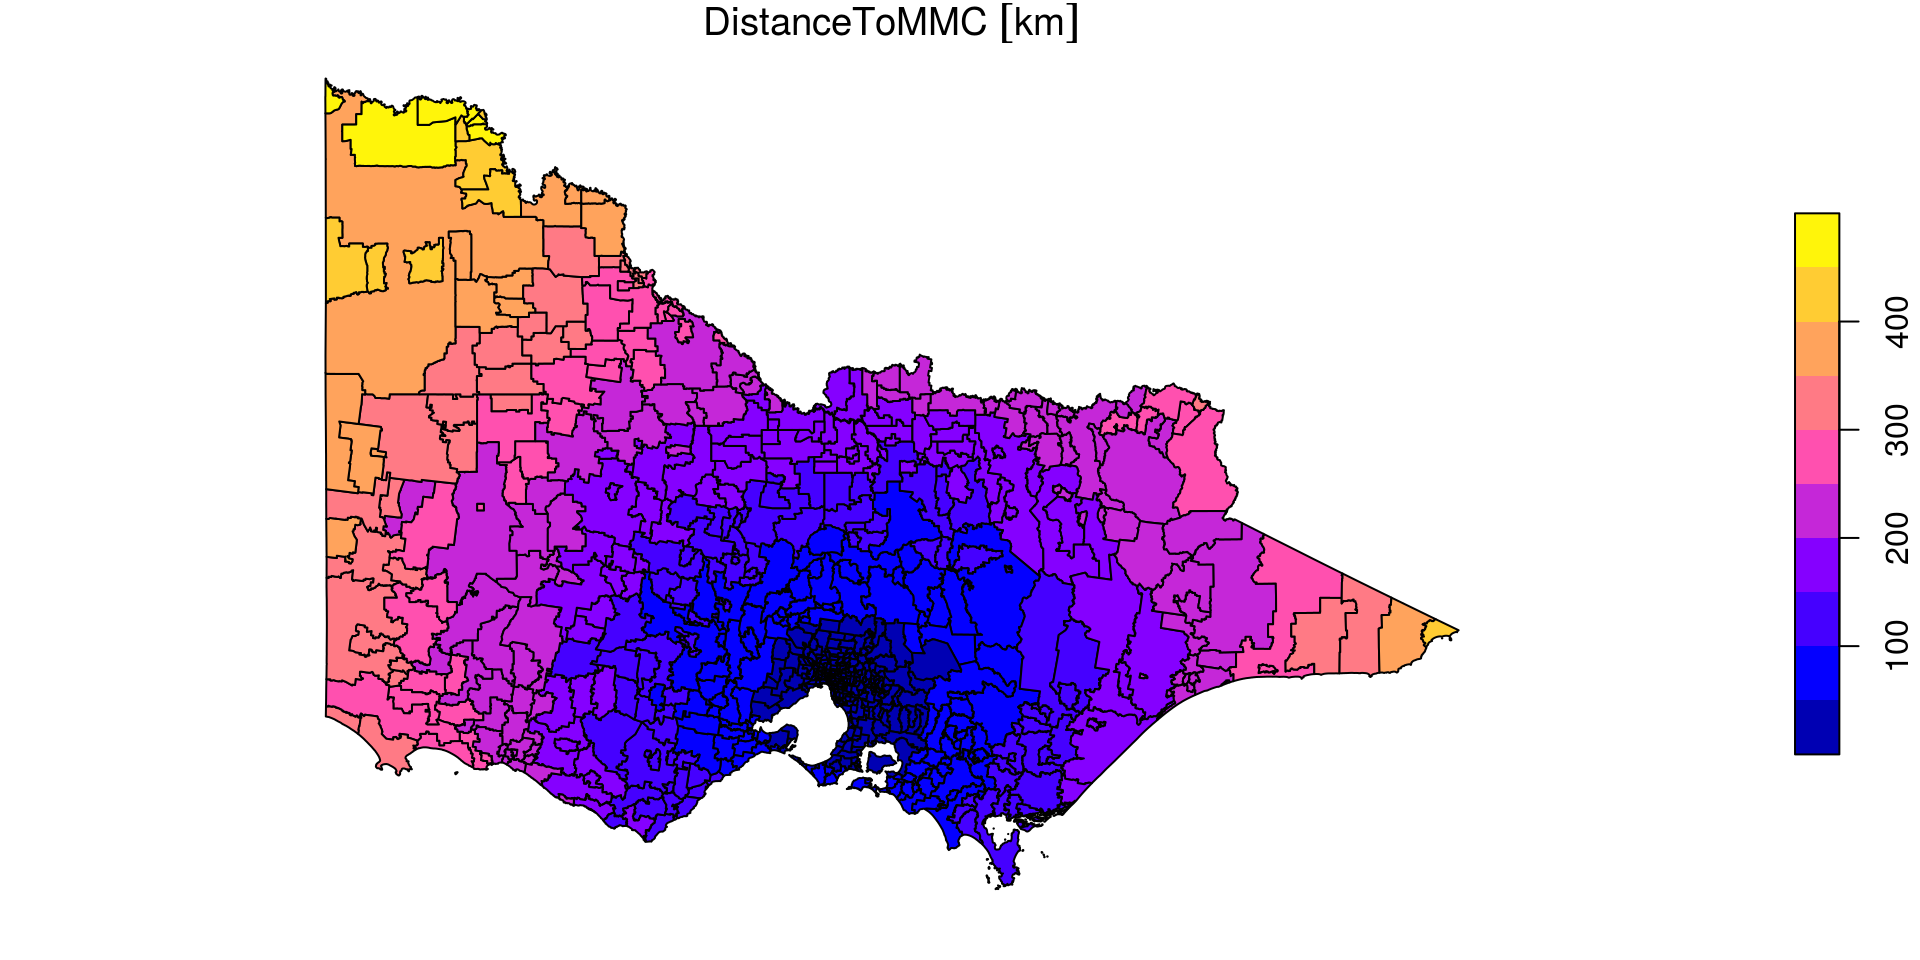
\includegraphics[width=10cm]{distance_mmc.png}
\end{center}
\caption{Visualization of straightline distance calculation from every postcode in the state to Monash Medical Centre. Static visualization created with {\em tmap}}\label{fig:DistanceToMMC}
\end{figure}

\begin{figure}[h!]
\begin{center}
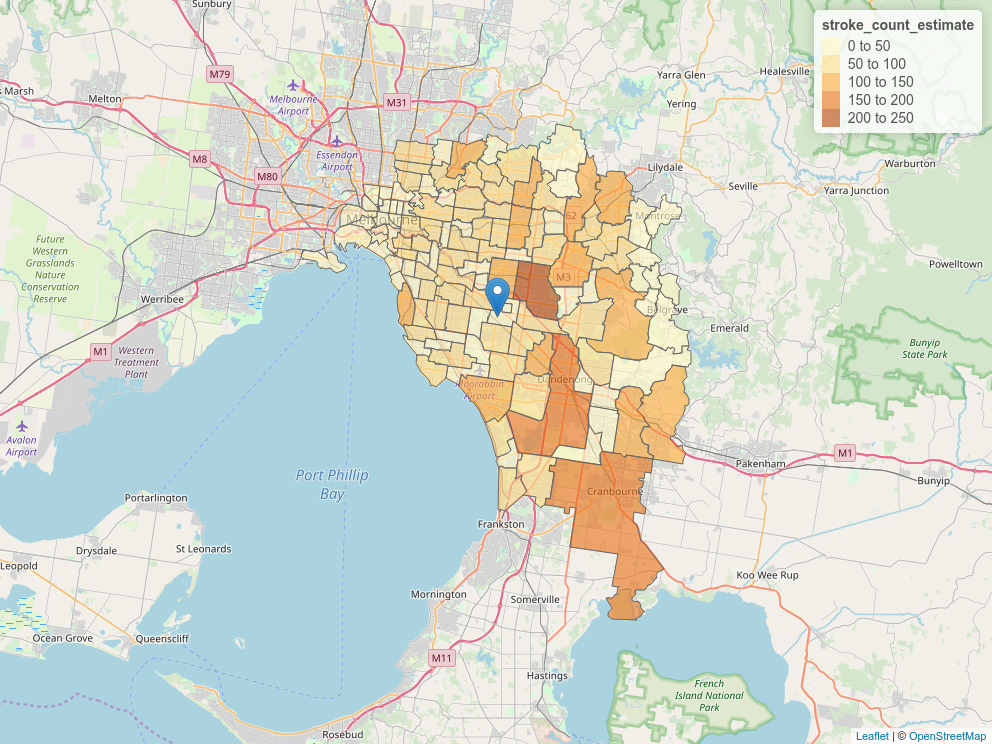
\includegraphics[width=10cm]{choropleth.png}
\end{center}
\caption{Choropleth of stroke case load estimate. Postcodes are coloured according to estimation of stroke cases derived from demographic data. Screenshot of interactive visualization created with {\em tmap}}\label{fig:choropleth}
\end{figure}

\begin{figure}[h!]
\begin{center}
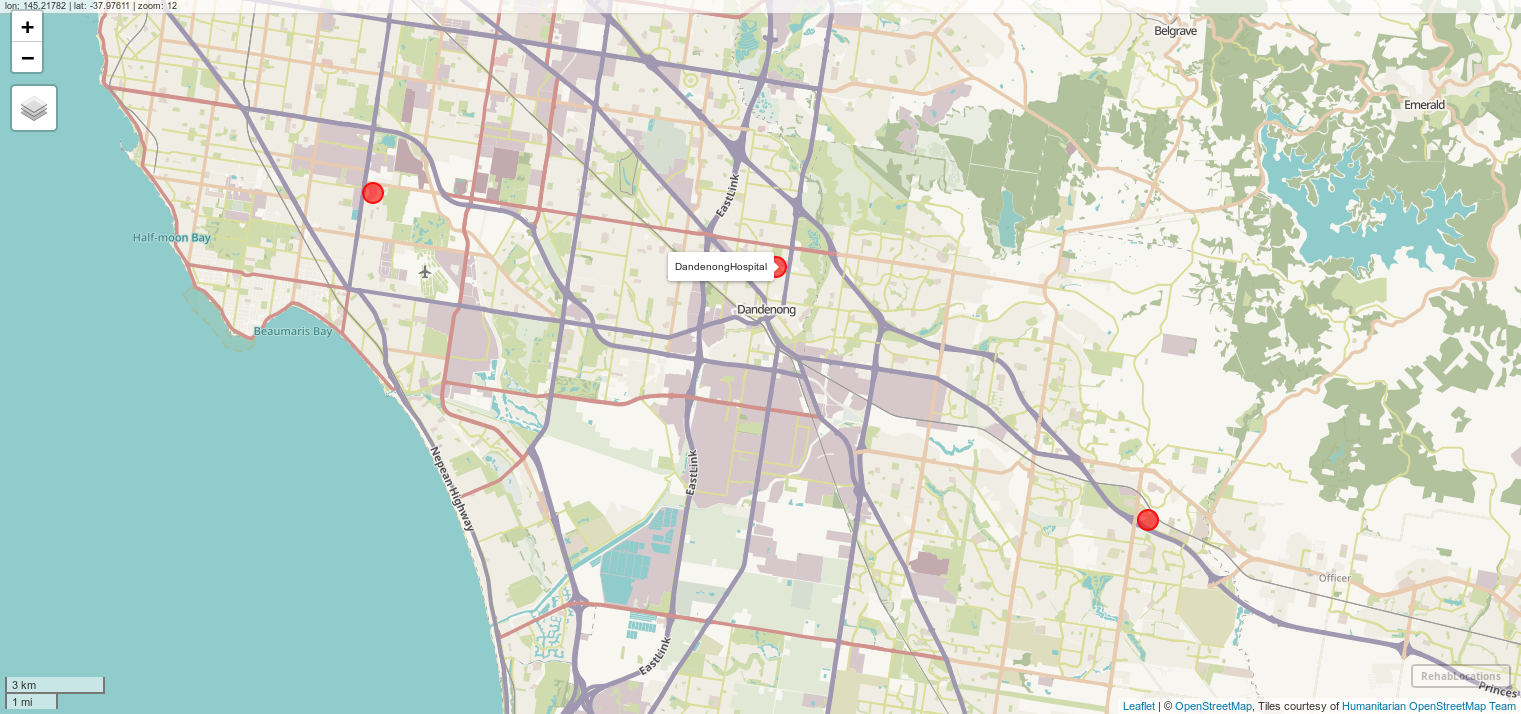
\includegraphics[width=12cm]{map1_mv.png}
\end{center}
\caption{Locations of the three rehabilitation centers determined by geocoding. Screenshot of interactive visualization created with {\em mapview}}\label{fig:RehabCenterLocations}
\end{figure}

\begin{figure}[h!]
\begin{center}
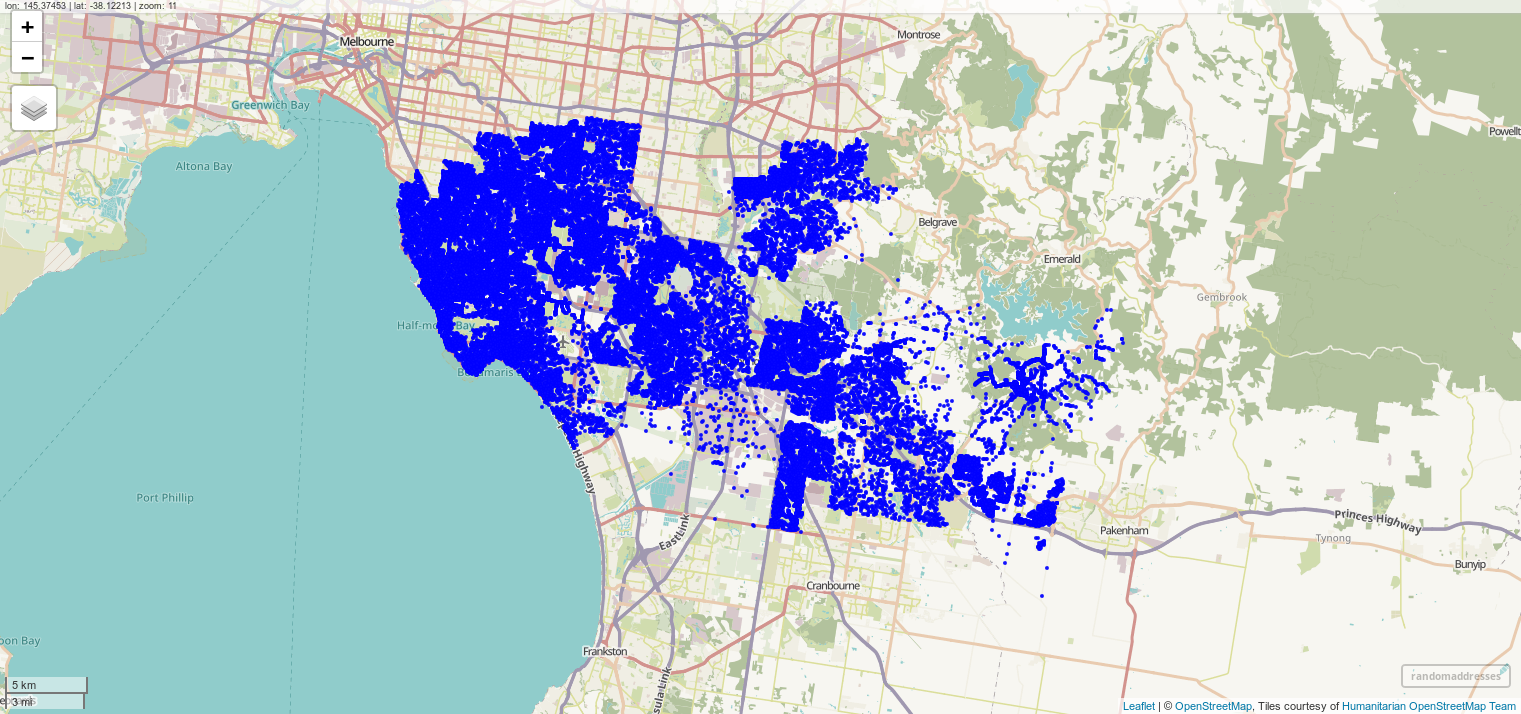
\includegraphics[width=12cm]{map2_mv.png}
\end{center}
\caption{Randomly sampled addresses within the postcodes of interest. 1000 addresses per postcode were sampled, and the differing population density across the postcodes of interest is clearly visible. Screenshot of interactive visualization created with {\em mapview}}\label{fig:RehabCenterRandomAddresses}
\end{figure}

\begin{figure}[h!]
\begin{center}
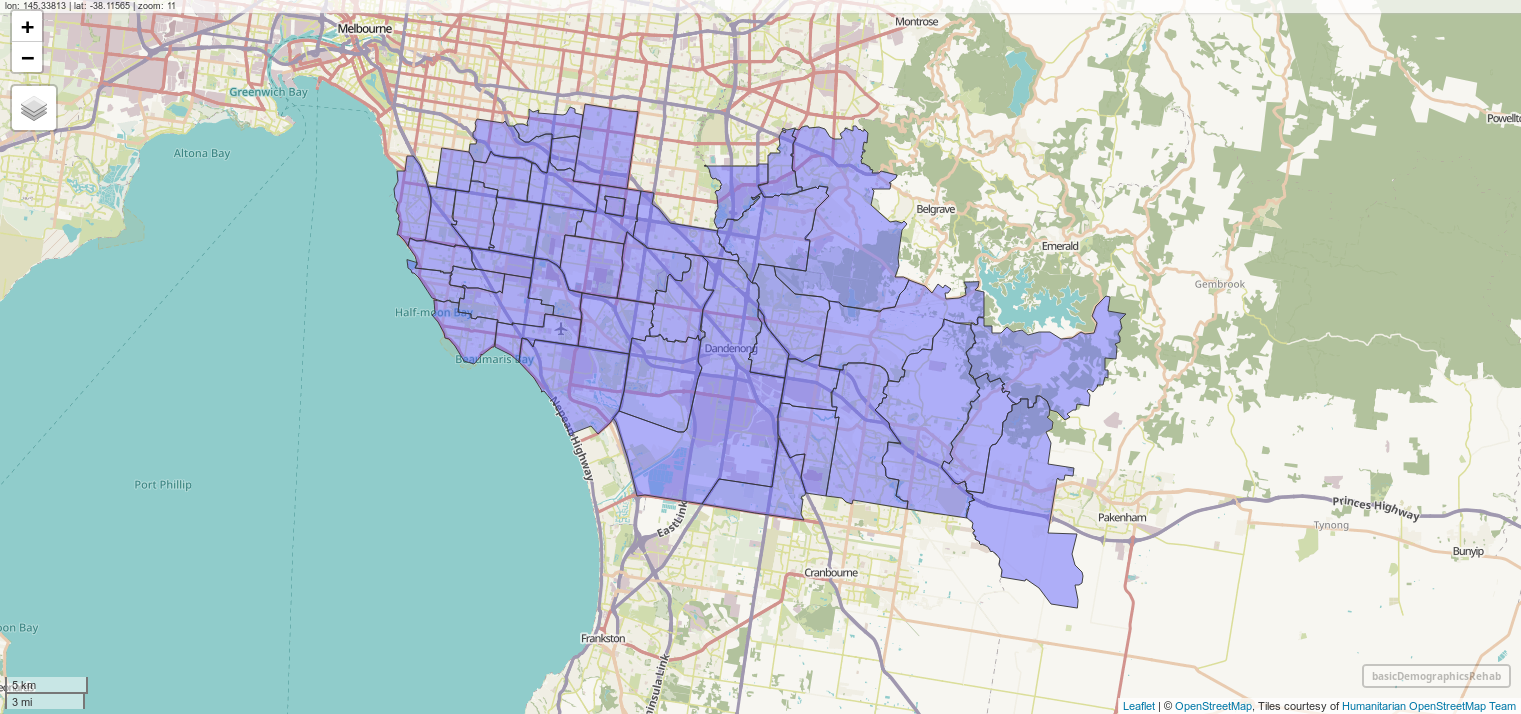
\includegraphics[width=12cm]{map3_mv.png}
\end{center}
\caption{Boundaries of postcodes with centroids within 10km of one of the
  rehabilitation centers. Screenshot of interactive visualization created with {\em mapview}}\label{fig:RehabCenterPostcodes}
\end{figure}

\begin{figure}[h!]
\begin{center}
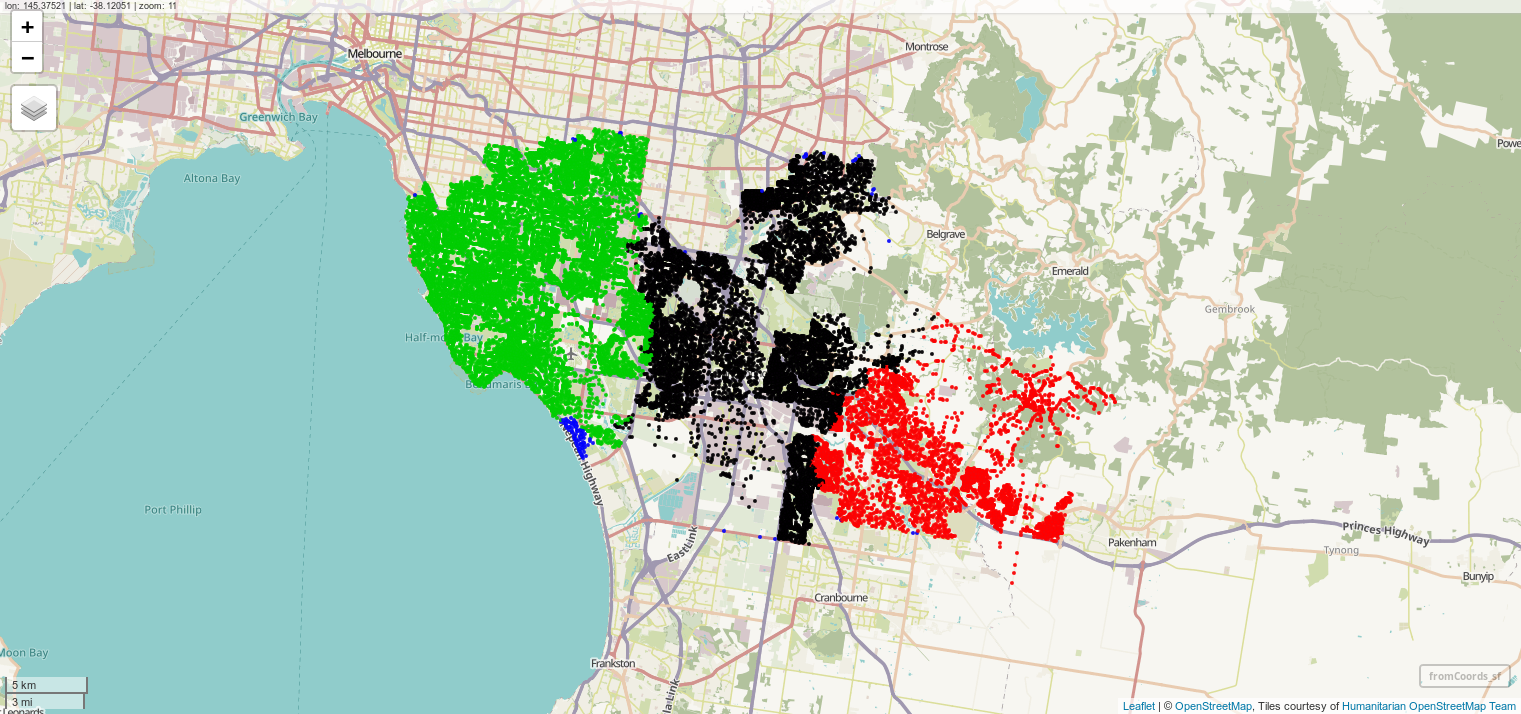
\includegraphics[width=12cm]{map4_mv.png}
\end{center}
\caption{Sampled address colourcoded according to nearest destination, with distance to destination computed through the street network. Screenshot of interactive visualization created with {\em mapview}}\label{fig:RehabCenterAddressCatchments}
\end{figure}

\begin{figure}[h!]
\begin{center}
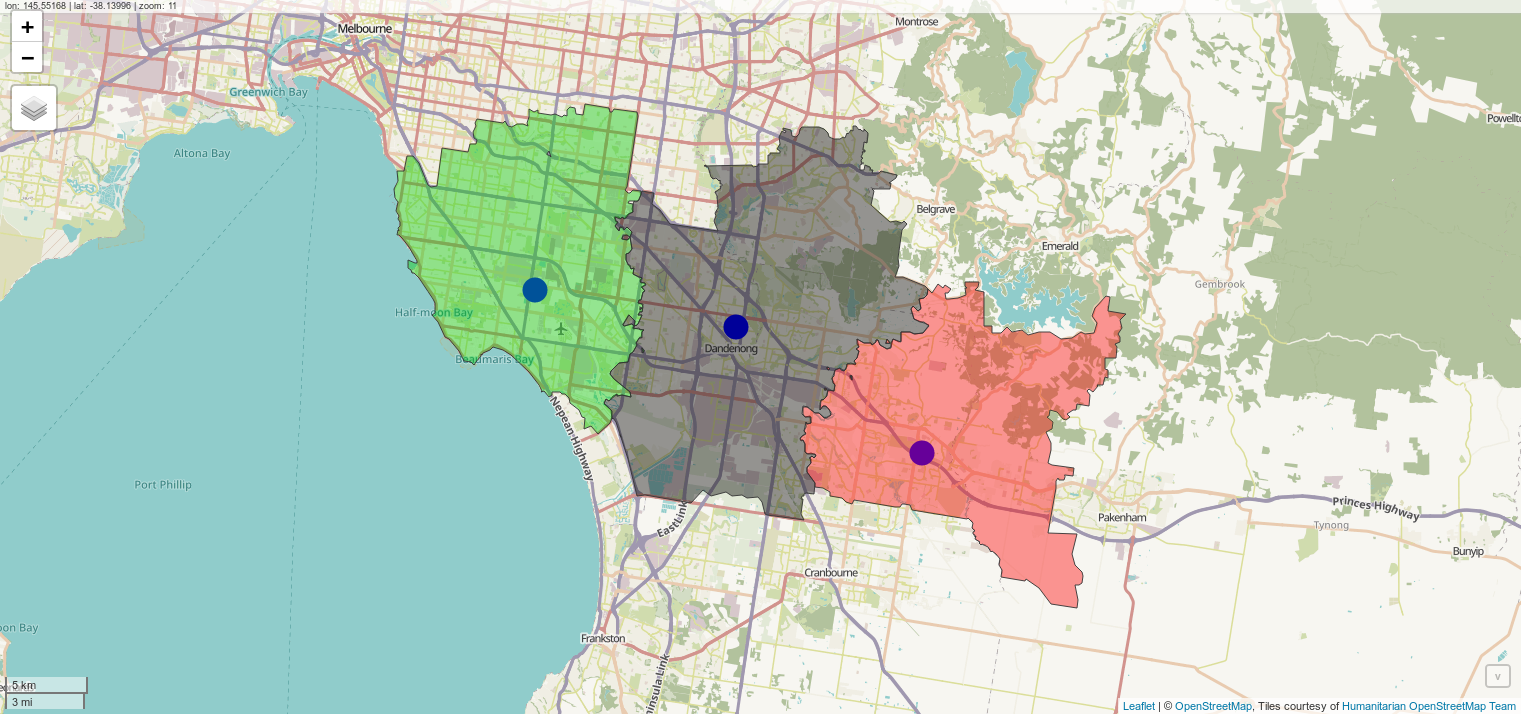
\includegraphics[width=12cm]{map5_mv.png}
\end{center}
\caption{Polygon representation of rehabilitation center catchment zones. Screenshot of interactive visualization created with {\em mapview}}\label{fig:RehabCenterPolyCatchments}
\end{figure}

\begin{figure}[h!]
\begin{center}
%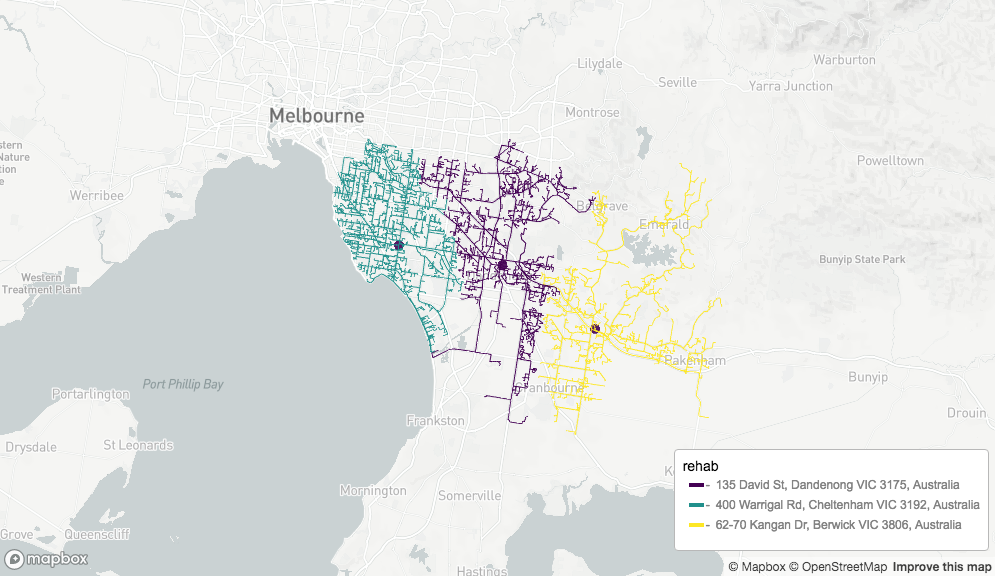
\includegraphics[width=10cm]{nearest_rehab.png}
\end{center}
\caption{Road network-based visualization of catchment zones for rehabilitation centers. Screenshot of interactive visualization created with {\em mapdeck} (API key required)}\label{fig:RehabCenterRoadCatchment}
\end{figure}

\begin{figure}[h!]
\begin{center}
%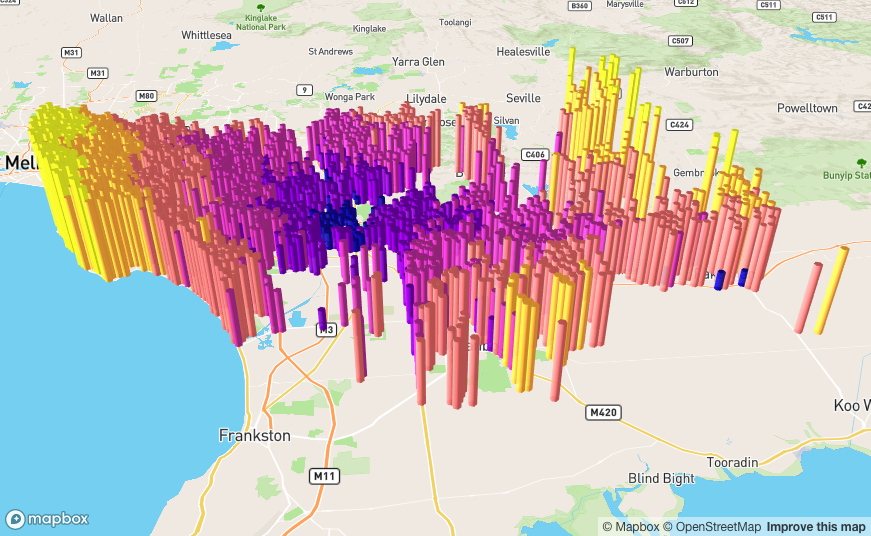
\includegraphics[width=10cm]{directions_rehab1_sample_mapdeck_hexagons.png}
\end{center}
\caption{Alternative visualization of distances from random addresses to rehabilitation centeres. Screenshot of interactive visualization created with {\em mapdeck} (API key required)}\label{fig:RehabCenterAddressDistanceHex}
\end{figure}

\begin{figure}[h!]
\begin{center}
%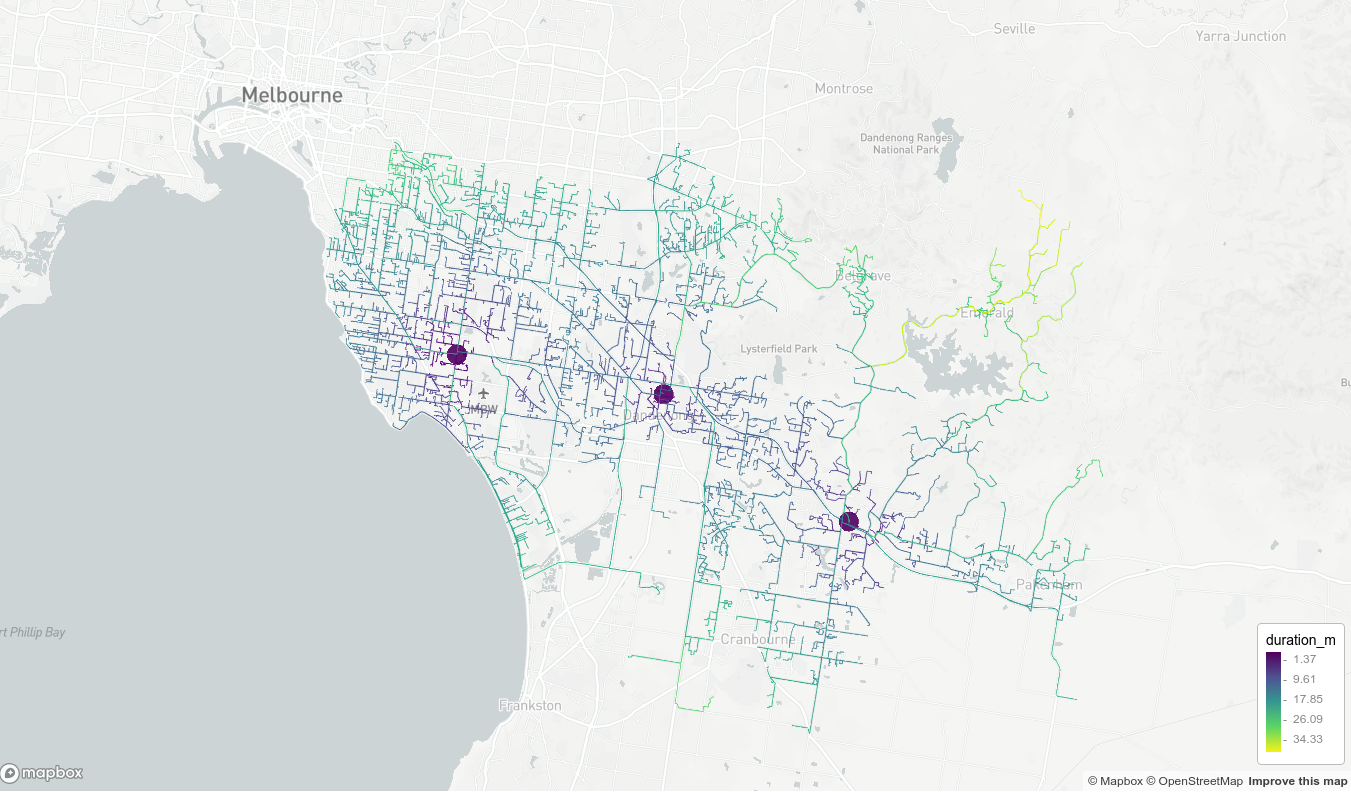
\includegraphics[width=10cm]{duration_all_rehab.png}
\end{center}
\caption{Road network visualization of travel times from random addresses to rehabilitation centeres. Screenshot of interactive visualization created with {\em mapdeck} (API key required)}\label{fig:RehabCenterAddressDistance}
\end{figure}


\bibliographystyle{frontiersinHLTHFPHY}
\bibliography{references}
\end{document}
